% !TeX root = ../main.tex

\chapter{问题定义与系统总体架构}
\label{cha:problem}

\section{问题定义}
\label{sec:problem-definition}

本文考虑如下自动驾驶感知任务。给定前视相机图像 $I$ 与问题描述 $q$，系统需要输出结构化结果 $y$，其中既包括问答标签，也包括场景三元组、动作建议与路由元信息。与只输出自然语言答案的方案不同，本文要求系统保留可供后续评测与复用的中间状态。因此，最终输出可表示为
\begin{equation}
  y = \{a, \mathcal{T}, u, m\},
\end{equation}
其中 $a$ 为最终问答答案，$\mathcal{T}$ 为结构化场景三元组集合，$u$ 为推荐动作，$m$ 为时延、技能匹配、候选标签分布等元数据。

边缘端模型首先生成候选标签分布 $p = \{p_1,\ldots,p_K\}$。本文使用熵作为不确定性代理量：
\begin{equation}
  H(p) = -\sum_{i=1}^{K} p_i \log p_i.
\end{equation}
当熵值较高，或模型触发回退标签，或命中已知长尾模式时，系统有理由认为当前结果存在进一步纠正的必要。

\section{研究假设与目标}
\label{sec:problem-hypothesis}

围绕本文的主问题，研究假设可表述为：

\begin{enumerate}
  \item \textbf{H1}：边缘端小型 VLM 在距离敏感的交通感知任务上存在显著 long-range degradation，尤其容易对 far-distance 的正样本产生假阴性。
  \item \textbf{H2}：云端大模型能够在远距离失败样本上提供更高上限，但其高时延使其不适合作为默认主链路，因此更合理的方式是 selective cloud routing，而不是 full cloud replacement。
  \item \textbf{H3}：在冻结主模型权重的条件下，系统仍然可以通过反思、检索与结构化 skill 复用形成测试时适配能力。
\end{enumerate}

基于上述假设，本文的系统优化目标可以概括为：
\begin{equation}
  \max \ \text{Acc}_{\text{final}} \quad \text{s.t.} \quad \text{CallRate}_{\text{cloud}} \le \tau_c,\ \text{Latency}_{\text{mean}} \le \tau_l.
\end{equation}
其中 $\tau_c$ 与 $\tau_l$ 分别表示可接受的云调用预算与平均时延预算。该目标明确表明，本文不是单纯追求准确率最大化，而是追求部署约束下的综合收益。

\section{系统总体架构}
\label{sec:problem-architecture}

本文系统由边缘感知器、云端反思器、技能库与编排器四个核心部分组成，其整体结构如图~\ref{fig:architecture} 所示。边缘端负责高频基础感知，云端负责低频定向纠错，skill store 负责沉淀外部知识，MCP 接口负责在各组件之间传递统一格式的请求与响应。

\begin{figure}[htbp]
  \centering
  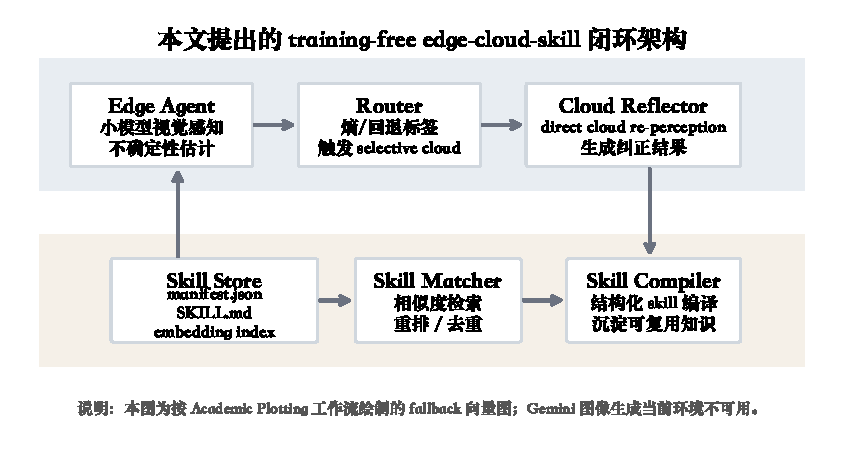
\includegraphics[width=0.95\textwidth]{image/thesis/fig_architecture.pdf}
  \bicaption{系统总体架构图}{System overview of the proposed hierarchical edge-cloud perception framework}
  \label{fig:architecture}
\end{figure}

图~\ref{fig:architecture} 体现了本文架构的三个关键设计：

\begin{enumerate}
  \item \textbf{角色分层}：边缘端与云端承担不同角色，而非简单的主备切换。
  \item \textbf{知识外化}：纠错经验通过 skill 编译进入外部存储，而不是立即改写模型参数。
  \item \textbf{协议统一}：所有中间状态均以结构化对象形式流转，便于记录、评测与复用。
\end{enumerate}

\section{系统执行流程}
\label{sec:problem-workflow}

系统执行流程如图~\ref{fig:workflow} 所示。对于单个样本，系统首先执行边缘端 baseline perception；若当前样本命中已有 skill，则执行带技能约束的再感知；若仍不满足稳定性条件，则触发 direct cloud re-perception；随后云端结果被整理为最终输出，并可进一步被编译为新的结构化 skill。

\begin{figure}[htbp]
  \centering
  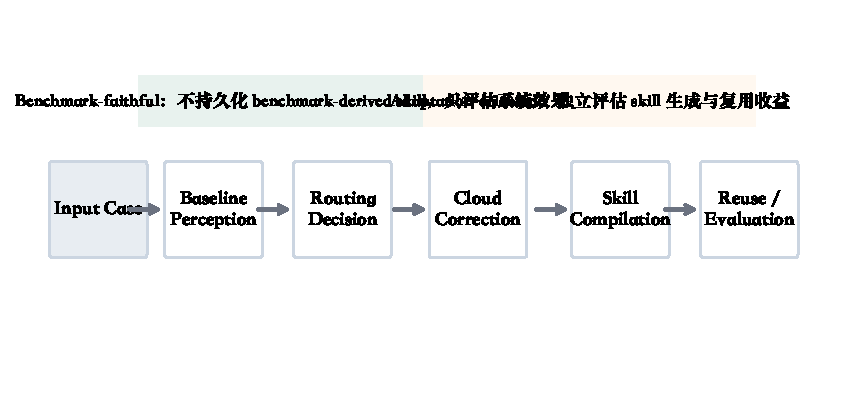
\includegraphics[width=0.95\textwidth]{image/thesis/fig_workflow.pdf}
  \bicaption{系统执行流程图}{Execution workflow from baseline perception to routing, correction, and skill reuse}
  \label{fig:workflow}
\end{figure}

上述流程与传统“边缘失败后直接回退云端答案”的做法存在本质差别。本文将云端视为反思与纠错节点，而不是默认主链路；同时，系统保留从当前样本中学习外部技能的能力，以便为后续样本提供更低成本的复用路径。

\section{路由策略}
\label{sec:problem-routing}

本文采用基于规则与不确定性代理量的混合路由策略。记输入样本为 $x$，则路由函数可写为
\begin{equation}
  R(x)=
  \begin{cases}
    \texttt{edge\_pass}, & \text{若 } H(p) < \tau_h \land \neg f(x) \land \neg g(x),\\
    \texttt{cloud\_reflect}, & \text{否则},
  \end{cases}
\end{equation}
其中 $\tau_h$ 为熵阈值，$f(x)$ 表示回退标签触发，$g(x)$ 表示与已知长尾失败模式相关的规则触发条件，例如 far-distance pedestrian presence 问题。采用该策略的原因在于，自动驾驶中的失败往往不是随机分布，而是与距离、局部目标尺寸和场景上下文紧密相关。

\section{证据分层与论文叙事边界}
\label{sec:problem-evidence}

为保证论文结论与证据强度一致，本文将全部结果划分为三层。

\begin{enumerate}
  \item \textbf{一级强结论}：以 \texttt{DTP-Synth / Category 1} clean 50-sample 三路对比为核心证据，用于证明 selective cloud routing 的系统有效性。
  \item \textbf{二级机制结论}：以独立 adaptation-oriented skill 实验为核心证据，用于说明结构化 skill 在测试时自适应中的潜力与风险。
  \item \textbf{三级观察结论}：以 \texttt{DTP-Real / Category 1} pilot 为核心证据，用于分析真实数据下的 far-collapse 与 false-negative bias，而不将其表述为最终普适结论。
\end{enumerate}

这种分层叙事既是本文写作规范的一部分，也是系统研究的重要方法论：只有在证据来源、协议边界和结论强度一致时，自动驾驶系统论文才能保持可信度。

\section{本章小结}
\label{sec:problem-summary}

本章从研究假设、优化目标、系统架构、执行流程与证据分层五个方面完成了问题定义。后续章节将在此基础上继续展开方法设计与系统实现，重点说明各模块如何在不更新主模型权重的前提下协同工作。
